\documentclass[10pt]{article}

\usepackage[text={14cm,20cm}]{geometry}
%\usepackage{mathtext}
\usepackage{amsmath,amssymb,amsthm,amscd,amsfonts}

\usepackage[utf8x]{inputenc}
%\usepackage{cmap}
\usepackage[T2A]{fontenc}
\usepackage[russian]{babel}
%\usepackage{lmodern}


\usepackage{euscript}
\usepackage{relsize}
\usepackage{mathdots}
\usepackage{graphicx}
%\usepackage{epstopdf}
%\usepackage{caption2}
\usepackage{indentfirst}
%\usepackage{fancyhdr}
%\usepackage{sectsty}
%\usepackage{titlesec}
% \usepackage{bbold}
\usepackage{tikz}
\usetikzlibrary{arrows.meta}
\usepackage{empheq}

\newcommand*\widefbox[1]{\fbox{\hspace{2em}#1\hspace{2em}}}

\usepackage[colorlinks, urlcolor=blue, pdfborder={0 0 0 [0 0]}]{hyperref}

\hyphenation{Struc-tu-red}
\hyphenation{Ran-do-mized}
\hyphenation{Ma-xi-mi-za-tion}
\DeclareMathOperator*{\argmax}{arg\,max}
\DeclareMathOperator*{\argmin}{arg\,min}
\DeclareMathOperator{\tr}{tr}
\providecommand*{\BibDash}{}

\def\rank{\mathop{\mathrm{rank}}}
\DeclareSymbolFont{bbold}{U}{bbold}{m}{n}
\DeclareSymbolFontAlphabet{\mathbbold}{bbold}

\newtheorem{corollary}{Следствие}
\newtheorem{proposition}{Предложение}
\newtheorem{algorithm}{Алгоритм}
\newtheorem{theorem}{Теорема}
\newtheorem{lemma}{Лемма}
\newtheorem{remark}{Замечание}
\newtheorem{problem}{Задача}

\usepackage{euscript}
\newcommand{\bt}{\begin{theorem}}
\newcommand{\et}{\end{theorem}}
\newcommand{\bl}{\begin{lemma}}
\newcommand{\el}{\end{lemma}}
\newcommand{\bp}{\begin{proposition}}
\newcommand{\ep}{\end{proposition}}
\newcommand{\bc}{\begin{corollary}}
\newcommand{\ec}{\end{corollary}}

\newcommand{\bd}{\begin{definition}\rm}
\newcommand{\ed}{\end{definition}}
\newcommand{\bex}{\begin{example}\rm}
\newcommand{\eex}{\end{example}}
\newcommand{\br}{\begin{remark}\rm}
\newcommand{\er}{\end{remark}}

\newcommand{\btbh}{\begin{table}[!ht]}
\newcommand{\etb}{\end{table}}
\newcommand{\bfgh}{\begin{figure}[!ht]}
\newcommand{\efg}{\end{figure}}

\newcommand{\bea}{\begin{eqnarray*}}
\newcommand{\eea}{\end{eqnarray*}}
\newcommand{\be}{\begin{eqnarray}}
\newcommand{\ee}{\end{eqnarray}}
%
\newcommand{\intl}{\int\limits}
\newcommand{\suml}{\sum\limits}
\newcommand{\liml}{\lim\limits}
\newcommand{\prodl}{\prod\limits}
\newcommand{\minl}{\min\limits}
\newcommand{\maxl}{\max\limits}
\newcommand{\supl}{\sup\limits}
%
\newcommand{\ve}{\varepsilon}
\newcommand{\vphi}{\varphi}
\newcommand{\ovl}{\overline}
\newcommand{\lm}{\lambda}
\def\wtilde{\widetilde}
\def\what{\widehat}

\newcommand{\ra}{\rightarrow}
\newcommand{\towith}[1]{\mathrel{\mathop{\longrightarrow}_{#1}}}

\def\bproof{\textbf{Proof.\ }}
\def\eproof{\hfill$\Box$\smallskip}

\def\spaceN{\mathsf{N}}
\def\spaceZ{\mathsf{Z}}
\def\spaceR{\mathsf{R}}
\def\spaceC{\mathsf{C}} %is not used?
\newcommand\Expect{\mathsf{E}}
%\newcommand\Variance{\mathsf{D}}

\newcommand{\bfw}{\mathbf{w}}

\def\last#1{{\underline{#1}}}
\def\llast#1{\underline{\underline{#1}}}
\def\first#1{{\mathstrut\overline{#1}}}
\def\ffirst#1{\mathstrut\overline{\mathstrut\overline{#1}}}
\def\overo#1{\overset{_\mathrm{o}}{#1}}
\newcommand{\ontop}[2]{\genfrac{}{}{0pt}{0}{#1}{#2}}
\def\bfpi{\mbox{\boldmath{$\pi$}}}
\def\bfmu{\mbox{\boldmath{$\mu$}}}
\def\bfPi{\mbox{\boldmath{$\Pi$}}}
\def\bfcR{\mbox{\boldmath{$\cR$}}}

\def\mmod{\mathop{\mathrm{mod}}}
\def\sspan{\mathop{\mathrm{span}}}
\def\rank{\mathop{\mathrm{rank}}}
\def\dist{\mathop{\mathrm{dist}}}

\newcommand{\reverse}{\mathop{\mathrm{rev}}}
\newcommand{\Arg}{\mathop\mathrm{Arg}}
\newcommand{\meas}{\mathop{\mathrm{meas}}}

\newcommand{\colspace}{\mathop{\mathrm{colspace}}}
\newcommand{\rowspace}{\mathop{\mathrm{rowspace}}}


\makeatletter
\def\adots{\mathinner{\mkern2mu\raise\p@\hbox{.}
\mkern2mu\raise4\p@\hbox{.}\mkern1mu
\raise7\p@\vbox{\kern7\p@\hbox{.}}\mkern1mu}}
\newcommand{\l@abcd}[2]{\hbox to\textwidth{#1\dotfill #2}}
\makeatother

\def\func{\mathop\mathrm}

% Some new definitions
\newcommand{\defeq}{\stackrel{def}{=}}
\newcommand{\frob}{\calF}
\def\trajmat#1{\calT_{\mathrm{#1}}}

\def\unit{\mathfrak{i}}


%new calligraphic font for subspaces
\usepackage{euscript}
\newcommand{\spA}{\EuScript{A}}
\newcommand{\spB}{\EuScript{B}}
\newcommand{\spC}{\EuScript{C}}
\newcommand{\spD}{\EuScript{D}}
\newcommand{\spE}{\EuScript{E}}
\newcommand{\spF}{\EuScript{F}}
\newcommand{\spG}{\EuScript{G}}
\newcommand{\spH}{\EuScript{H}}
\newcommand{\spI}{\EuScript{I}}
\newcommand{\spJ}{\EuScript{J}}
\newcommand{\spK}{\EuScript{K}}
\newcommand{\spL}{\EuScript{L}}
\newcommand{\spM}{\EuScript{M}}
\newcommand{\spN}{\EuScript{N}}
\newcommand{\spO}{\EuScript{O}}
\newcommand{\spP}{\EuScript{P}}
\newcommand{\spQ}{\EuScript{Q}}
\newcommand{\spR}{\EuScript{R}}
\newcommand{\spS}{\EuScript{S}}
\newcommand{\spT}{\EuScript{T}}
\newcommand{\spU}{\EuScript{U}}
\newcommand{\spV}{\EuScript{V}}
\newcommand{\spW}{\EuScript{W}}
\newcommand{\spX}{\EuScript{X}}
\newcommand{\spY}{\EuScript{Y}}
\newcommand{\spZ}{\EuScript{Z}}

%font for text indices like transposition X^\mathrm{T}
\newcommand{\rmA}{\mathrm{A}}
\newcommand{\rmB}{\mathrm{B}}
\newcommand{\rmC}{\mathrm{C}}
\newcommand{\rmD}{\mathrm{D}}
\newcommand{\rmE}{\mathrm{E}}
\newcommand{\rmF}{\mathrm{F}}
\newcommand{\rmG}{\mathrm{G}}
\newcommand{\rmH}{\mathrm{H}}
\newcommand{\rmI}{\mathrm{I}}
\newcommand{\rmJ}{\mathrm{J}}
\newcommand{\rmK}{\mathrm{K}}
\newcommand{\rmL}{\mathrm{L}}
\newcommand{\rmM}{\mathrm{M}}
\newcommand{\rmN}{\mathrm{N}}
\newcommand{\rmO}{\mathrm{O}}
\newcommand{\rmP}{\mathrm{P}}
\newcommand{\rmQ}{\mathrm{Q}}
\newcommand{\rmR}{\mathrm{R}}
\newcommand{\rmS}{\mathrm{S}}
\newcommand{\rmT}{\mathrm{T}}
\newcommand{\rmU}{\mathrm{U}}
\newcommand{\rmV}{\mathrm{V}}
\newcommand{\rmW}{\mathrm{W}}
\newcommand{\rmX}{\mathrm{X}}
\newcommand{\rmY}{\mathrm{Y}}
\newcommand{\rmZ}{\mathrm{Z}}

%tt font for time series
\newcommand{\tsA}{\mathbb{A}}
\newcommand{\tsB}{\mathbb{B}}
\newcommand{\tsC}{\mathbb{C}}
\newcommand{\tsD}{\mathbb{D}}
\newcommand{\tsE}{\mathbb{E}}
\newcommand{\tsF}{\mathbb{F}}
\newcommand{\tsG}{\mathbb{G}}
\newcommand{\tsH}{\mathbb{H}}
\newcommand{\tsI}{\mathbb{I}}
\newcommand{\tsJ}{\mathbb{J}}
\newcommand{\tsK}{\mathbb{K}}
\newcommand{\tsL}{\mathbb{L}}
\newcommand{\tsM}{\mathbb{M}}
\newcommand{\tsN}{\mathbb{N}}
\newcommand{\tsO}{\mathbb{O}}
\newcommand{\tsP}{\mathbb{P}}
\newcommand{\tsQ}{\mathbb{Q}}
\newcommand{\tsR}{\mathbb{R}}
\newcommand{\tsS}{\mathbb{S}}
\newcommand{\tsT}{\mathbb{T}}
\newcommand{\tsU}{\mathbb{U}}
\newcommand{\tsV}{\mathbb{V}}
\newcommand{\tsW}{\mathbb{W}}
\newcommand{\tsX}{\mathbb{X}}
\newcommand{\tsY}{\mathbb{Y}}
\newcommand{\tsZ}{\mathbb{Z}}

%bf font for matrices
\newcommand{\bfA}{\mathbf{A}}
\newcommand{\bfB}{\mathbf{B}}
\newcommand{\bfC}{\mathbf{C}}
\newcommand{\bfD}{\mathbf{D}}
\newcommand{\bfE}{\mathbf{E}}
\newcommand{\bfF}{\mathbf{F}}
\newcommand{\bfG}{\mathbf{G}}
\newcommand{\bfH}{\mathbf{H}}
\newcommand{\bfI}{\mathbf{I}}
\newcommand{\bfJ}{\mathbf{J}}
\newcommand{\bfK}{\mathbf{K}}
\newcommand{\bfL}{\mathbf{L}}
\newcommand{\bfM}{\mathbf{M}}
\newcommand{\bfN}{\mathbf{N}}
\newcommand{\bfO}{\mathbf{O}}
\newcommand{\bfP}{\mathbf{P}}
\newcommand{\bfQ}{\mathbf{Q}}
\newcommand{\bfR}{\mathbf{R}}
\newcommand{\bfS}{\mathbf{S}}
\newcommand{\bfT}{\mathbf{T}}
\newcommand{\bfU}{\mathbf{U}}
\newcommand{\bfV}{\mathbf{V}}
\newcommand{\bfW}{\mathbf{W}}
\newcommand{\bfX}{\mathbf{X}}
\newcommand{\bfY}{\mathbf{Y}}
\newcommand{\bfZ}{\mathbf{Z}}

%bb font for standard spaces and expectation
\newcommand{\bbA}{\mathbb{A}}
\newcommand{\bbB}{\mathbb{B}}
\newcommand{\bbC}{\mathbb{C}}
\newcommand{\bbD}{\mathbb{D}}
\newcommand{\bbE}{\mathbb{E}}
\newcommand{\bbF}{\mathbb{F}}
\newcommand{\bbG}{\mathbb{G}}
\newcommand{\bbH}{\mathbb{H}}
\newcommand{\bbI}{\mathbb{I}}
\newcommand{\bbJ}{\mathbb{J}}
\newcommand{\bbK}{\mathbb{K}}
\newcommand{\bbL}{\mathbb{L}}
\newcommand{\bbM}{\mathbb{M}}
\newcommand{\bbN}{\mathbb{N}}
\newcommand{\bbO}{\mathbb{O}}
\newcommand{\bbP}{\mathbb{P}}
\newcommand{\bbQ}{\mathbb{Q}}
\newcommand{\bbR}{\mathbb{R}}
\newcommand{\bbS}{\mathbb{S}}
\newcommand{\bbT}{\mathbb{T}}
\newcommand{\bbU}{\mathbb{U}}
\newcommand{\bbV}{\mathbb{V}}
\newcommand{\bbW}{\mathbb{W}}
\newcommand{\bbX}{\mathbb{X}}
\newcommand{\bbY}{\mathbb{Y}}
\newcommand{\bbZ}{\mathbb{Z}}

%got font for any case
\newcommand{\gA}{\mathfrak{A}}
\newcommand{\gB}{\mathfrak{B}}
\newcommand{\gC}{\mathfrak{C}}
\newcommand{\gD}{\mathfrak{D}}
\newcommand{\gE}{\mathfrak{E}}
\newcommand{\gF}{\mathfrak{F}}
\newcommand{\gG}{\mathfrak{G}}
\newcommand{\gH}{\mathfrak{H}}
\newcommand{\gI}{\mathfrak{I}}
\newcommand{\gJ}{\mathfrak{J}}
\newcommand{\gK}{\mathfrak{K}}
\newcommand{\gL}{\mathfrak{L}}
\newcommand{\gM}{\mathfrak{M}}
\newcommand{\gN}{\mathfrak{N}}
\newcommand{\gO}{\mathfrak{O}}
\newcommand{\gP}{\mathfrak{P}}
\newcommand{\gQ}{\mathfrak{Q}}
\newcommand{\gR}{\mathfrak{R}}
\newcommand{\gS}{\mathfrak{S}}
\newcommand{\gT}{\mathfrak{T}}
\newcommand{\gU}{\mathfrak{U}}
\newcommand{\gV}{\mathfrak{V}}
\newcommand{\gW}{\mathfrak{W}}
\newcommand{\gX}{\mathfrak{X}}
\newcommand{\gY}{\mathfrak{Y}}
\newcommand{\gZ}{\mathfrak{Z}}

%old calligraphic font
\newcommand{\calA}{\mathcal{A}}
\newcommand{\calB}{\mathcal{B}}
\newcommand{\calC}{\mathcal{C}}
\newcommand{\calD}{\mathcal{D}}
\newcommand{\calE}{\mathcal{E}}
\newcommand{\calF}{\mathcal{F}}
\newcommand{\calG}{\mathcal{G}}
\newcommand{\calH}{\mathcal{H}}
\newcommand{\calI}{\mathcal{I}}
\newcommand{\calJ}{\mathcal{J}}
\newcommand{\calK}{\mathcal{K}}
\newcommand{\calL}{\mathcal{L}}
\newcommand{\calM}{\mathcal{M}}
\newcommand{\calN}{\mathcal{N}}
\newcommand{\calO}{\mathcal{O}}
\newcommand{\calP}{\mathcal{P}}
\newcommand{\calQ}{\mathcal{Q}}
\newcommand{\calR}{\mathcal{R}}
\newcommand{\calS}{\mathcal{S}}
\newcommand{\calT}{\mathcal{T}}
\newcommand{\calU}{\mathcal{U}}
\newcommand{\calV}{\mathcal{V}}
\newcommand{\calW}{\mathcal{W}}
\newcommand{\calX}{\mathcal{X}}
\newcommand{\calY}{\mathcal{Y}}
\newcommand{\calZ}{\mathcal{Z}}

%sf font for transposition and spaces like R
\newcommand{\sfA}{\mathsf{A}}
\newcommand{\sfB}{\mathsf{B}}
\newcommand{\sfC}{\mathsf{C}}
\newcommand{\sfD}{\mathsf{D}}
\newcommand{\sfE}{\mathsf{E}}
\newcommand{\sfF}{\mathsf{F}}
\newcommand{\sfG}{\mathsf{G}}
\newcommand{\sfH}{\mathsf{H}}
\newcommand{\sfI}{\mathsf{I}}
\newcommand{\sfJ}{\mathsf{J}}
\newcommand{\sfK}{\mathsf{K}}
\newcommand{\sfL}{\mathsf{L}}
\newcommand{\sfM}{\mathsf{M}}
\newcommand{\sfN}{\mathsf{N}}
\newcommand{\sfO}{\mathsf{O}}
\newcommand{\sfP}{\mathsf{P}}
\newcommand{\sfQ}{\mathsf{Q}}
\newcommand{\sfR}{\mathsf{R}}
\newcommand{\sfS}{\mathsf{S}}
\newcommand{\sfT}{\mathsf{T}}
\newcommand{\sfU}{\mathsf{U}}
\newcommand{\sfV}{\mathsf{V}}
\newcommand{\sfW}{\mathsf{W}}
\newcommand{\sfX}{\mathsf{X}}
\newcommand{\sfY}{\mathsf{Y}}
\newcommand{\sfZ}{\mathsf{Z}}

%\sectionfont{\centering}

%\subsectionfont{\centering}
%\subsubsectionfont{\normalsize}
%\setcounter{page}{1}


\author{Звонарев Никита}
\title{О поиске весов в задаче взвешенной аппроксимации рядом конечного ранга}
\begin{document}
\maketitle

\section*{Введение}
Рассмотрим задачу извлечения сигнала $\tsS~=~(s_1, \ldots, s_N)$ из зашумлённого временного ряда $\tsX = \tsS + \tsN$, где $\tsS$ управляется \emph{линейной рекуррентной формулой} (ЛРФ) порядка $r$: $s_n = \sum_{i = 1}^{r} a_i s_{n-i}$, $n = r + 1, \ldots, N$, $a_r\neq 0$. Ряды, управляемые ЛРФ, могут быть записаны в параметрическом виде $s_n = \sum_i P_i(n) \exp(\alpha_i n) \cos(2 \pi \omega_i n + \psi_i)$, где $P_i(n)$ --- многочлены от $n$  \cite{Golyandina.etal2001}.

Известно \cite{Broomhead.King1986, Vautard.etal1992, Elsner.Tsonis1996, Golyandina.etal2001}, что для выделения такого рода сигналов хорошо работают методы, основанные на оценке сигнального подпространства (subspace-based methods). Идея методов состоит в следующем: зафиксируем \emph{длину окна} $L$, $1 < L < N$, положим $K = N - L + 1$, и определим \emph{траекторную матрицу} для ряда $\tsS \in \sfX_N$ ($\sfX_N$ --- множество вещественных временных рядов длины $N$):
\begin{equation*}
\bfS = \calT_L(\tsS) =  \begin{pmatrix}
s_1 & s_2 & \ldots & s_K \\
s_2 & s_3 & \ldots & s_{K + 1} \\
\vdots & \vdots & \vdots & \vdots \\
s_L & s_{L + 1} & \ldots & s_N
\end{pmatrix},
\end{equation*}
где $\calT_L$ обозначает биекцию между $\sfX_N$ и $\calH$ --- множество ганкелевых матриц порядка $L \times K$ с одинаковыми значениями на побочных диагоналях $i+j=\mathrm{const}$.
%Пусть $\tsS$ управляется ЛРФ порядка $r$, $r < \min(L, K)$, и не управляется ЛРФ меньшего порядка. Тогда $\rank \bfS = r$, и, таким образом, $\bfS$ --- ганкелева матрица неполного ранга $r$. Ряд $\tsS$, у которого траекторная матрица $\bfS$ имеет неполный ранг $r$, назовём \emph{рядом конечного ранга}. Пространство столбцов матрицы $\bfS$, то есть сигнальное подпространство, даёт оценки $\alpha_i$ и $\omega_i$ в \eqref{parametricform} с помощью метода ESPRIT \cite{Roy.Kailath1989, Golyandina.Zhigljavsky2012}, применённого к $\bfS$. К тому же, полученные оценки позволяют решать целое множество связанных задач: прогнозирование ряда, заполнение пропусков и так далее, см. \cite{Golyandina.etal2001}.
Скажем, что ряд $\tsS$, у которого траекторная матрица $\bfS$ имеет неполный ранг $r$, называется \emph{рядом конечного ранга} $r$, после чего рассмотрим задачу аппроксимации временного ряда рядом конечного ранга по взвешенной норме \cite{Zvonarev2015, Gillard2014}:
\begin{equation}\label{eq:sourcetask}
\sum_{i = 1}^N q_i (x_i - y_i)^2 \to \min_{\tsY: \rank \bfY  = \calT_L(\tsY) \le r},
\end{equation}
где $\tsX = (x_1, \ldots, x_N) \in \sfX_N$ --- исходный временной ряд, $\tsY = (y_1, \ldots, y_N)$ --- требуемая аппроксимация, $\bfY = \calT(\tsY)$ --- соответствующая траекторная матрица, $q_i > 0$, $i = 1, \ldots, N$ --- веса (в дальнейшем называемые ``весами ряда''). 
%Отображение $\calT$ работает следующим образом: для $\calT(\tsX) = \bfX$ $\hat x_{l, k} = x_{l + k - 1}$, где $\tsX = (x_1, \ldots, x_N)$, $\bfX = (\hat x_{l, k})$. 
Полученное решение $\tsY^\star$ задачи \eqref{eq:sourcetask} можно использовать как оценку сигнала $\tsS$ рядом конечного ранга. Более того, полученная оценка позволяет решить множество связанных задач: оценка коэффициентов ЛРФ и параметров ряда, прогнозирование ряда, заполнение пропусков и так далее, см. \cite{Golyandina.etal2001}.

Обозначим соответствующее скалярное произведение в $\sfX_N$ rкак $\langle \tsX, \tsY \rangle_q = \sum_{i=1}^N q_i x_i y_i$.  Для решения задачи \eqref{eq:sourcetask} в \cite{Zvonarev2015} рассматривается эквивалентная задача структурной аппроксимации матрицей неполного ранга (Structured Low-Rank Approximation, SLRA):
\begin{equation*}
	\|\bfX - \bfY\|^2_\bfC \to \min_{\substack{\rank \bfY \le r \\ \bfY \in \calH}},
\end{equation*}
где $\bfX = \calT(\tsX)$, а матричная норма $\|\cdot\|_\bfC$ ($\bfC$ --- диагональная, положительно определённая матрица) порождена следующим скалярным произведением:
\begin{equation*}
\langle \bfY, \bfZ \rangle_\bfC = \tr(\bfY \bfC \bfZ^\rmT) = \sum_{l=1}^L \sum_{k=1}^K c_k y_{l,k} z_{l, k},
\end{equation*}
где $\bfC = \diag(c_1, \ldots, c_K)$, $\bfY = (y_{l, k})$, $\bfZ = (z_{l, k})$. Между весами в задаче аппроксимации ряда $q_i$ и весами $c_i$ (в дальнейшем называемые ``матричными весами'') существует соотношение, см. \cite[Proposition 4]{Zvonarev2015} для эквивалентности норм.

Основная проблема состояла в том, чтобы получить $q_i = 1$ и использовать оценки ряда, полученные при решении задачи невзвешенных наименьших квадратов в пространстве рядов. Однако, опять же согласно \cite[Lemma 1]{Zvonarev2015} и \cite{Gillard2014}, если это и возможно, то только при вырожденной матрице $\bfC$, что недопустимо при решении задачи методами типа Oblique Cadzow, см. \cite[Remark 4]{Zvonarev2015}. Следовательно, равномерностью весов ряда $q_i$ приходится жертвовать, и использовать матричные веса $c_i$ такие, чтобы $\bfC$ была невырожденной, а веса $q_i$ лишь близкими к равномерным.

Цель статьи --- разработать эффективный алгоритм поиска весов при зафиксированной мере невырожденности матрицы $\bfC$. В качестве такой меры ограничим число обусловленности $\bfC$. Для того чтобы не допустить вырожденность матрицы , ограничим её число обусловленности. Так же, как и в \cite{Zvonarev2015}, введём параметр $0 < \alpha \le 1$, и потребуем, чтобы все $c_i \ge 0$ и
\begin{equation} \label{eq:ratiocond}
\frac{\min_i c_i}{\max_i c_i} \ge \alpha,
\end{equation}
что эквивалентно тому, что $\text{Сond}(\bfC) \le 1/\alpha$, после чего поставим задачу аппроксимации единичных весов ряда по наиболее естественной эвклидовой норме. В этом и состоит ключевое отличие от предыдущего подхода, описанного в \cite[Proposition 5]{Zvonarev2015} и неприменимого в большинстве практических ситуаций: например, ранее требовалось, чтобы длина ряда $N$ была кратной длиине окна $L$. С другой стороны, решение задачи в такой постановке сводится к использованию теории экстремальных задач и квадратичного программирования, и получение эффективного по скорости работы алгоритма поиска весов является нетривиальной задачей.

В \cite[Section 5]{Zvonarev2015} показано, что чем равномернее веса ряда в задаче \eqref{eq:sourcetask}, тем точнее получается решение. Более того, как было показано в \cite{Zvonarev2015}, параметр $\alpha$ влияет на скорость сходимости метода Oblique Cadzow: чем больше $\text{Сond}(\bfC)$ (что равнозначно меньшему значению $\alpha$), тем медленнее сходится метод. В Разделе \ref{sect:numeric} показано, что эти соотношения выполняются и для весов, полученных новым методом.

\tableofcontents
\section{Постановка задачи аппроксимации весов}
Для удобства переформулируем предложение \cite[Proposition 4]{Zvonarev2015}, связывающее $c_i$ и $q_i$, в матричном виде. Для этого рассмотрим матрицу $\bfB = (b_{i, j})$ порядка $N \times K$, имеющую следующий вид:
\begin{equation} \label{eq:tmatrix}
b_{i, j} = \begin{cases}
1, & \text{для} \; i = j, \ldots, j + L - 1, \\
0, & \text{в противном случае}.
\end{cases}
\end{equation}
Заметим, что матрица $\bfB$ полного ранга. Предложение выглядит следующим образом:
\begin{proposition}
	Пусть $\bfY = \calT(\tsY)$, $\bfZ = \calT(\tsZ)$, $Q = (q_1, \ldots, q_N)^\rmT$, $C = (c_1, \ldots, c_K)^\rmT$. Тогда $\langle \tsY, \tsZ \rangle_q = \langle \bfY, \bfZ \rangle_\bfC$ для любых $\tsY, \tsZ \in \sfX_n$ тогда и только тогда, когда $Q = \bfB C$.
\end{proposition}

В общем виде задачу аппроксимации весов cформулируем следующим образом:
\begin{problem}\label{problem:commonw}
\begin{subequations} 
\begin{empheq}[box=\widefbox]{gather}
%\begin{equation}
	\label{eq:commonw}
\varphi^\star = \min_{C \in \calC} \varphi(C), \quad \text{где} \quad \varphi(C) = \|\bfB C - \mathbbold{1}_N\|,\\
\calC = \left\lbrace c_i \ge 0, \quad i = 1, \ldots, K, \quad \label{eq:commonw_cond}
\frac{\min_i c_i}{\max_i c_i} \ge \alpha \right\rbrace, 
\end{empheq}
\end{subequations}
где $\mathbbold{1}_N = (1, \ldots, 1)^\rmT \in \sfR_N$ --- требуемые веса ряда (вектор из $N$ единиц), $0 < \alpha \le 1$ --- параметр, регулирующий степень вырожденности матрицы $\bfC$, $\|\cdot\|$ --- эвклидова норма в $\sfR^N$.
\end{problem}
%Рассмотрим следующие стандартные нормы:
% \begin{enumerate}
%	\item $\|X\| = \|X\|_2 = \sqrt{\sum_i x_i^2}$ --- обычная евклидова норма,
%	\item $\|X\| = \|X\|_\infty = \max_i |x_i|$,
%	\item $\|X\| = \|X\|_1 = \sum_i |x_i|$ --- норма, порождающая манхеттенскую метрику.
%\end{enumerate}
%
%\begin{remark}
%	В дальнейшем, мы рассмотрим только случай нормы $\|X\|_2$. В остальных случаях Задачу \ref{problem:commonw} можно решить с помощью линейного программирования, см. \cite{nocedal2006numerical}.
%\end{remark}

\section{Эквивалентные формулировки}
Раскроем функцию $\varphi^2(C)/2$ из \eqref{eq:commonw}, избавимся от константного члена и перепишем множество $\calC$ из \eqref{eq:commonw_cond} в виде набора линейных ограничений. Получим следующую эквивалентную формулировку:
\begin{problem} \label{problem:quadtf}
\begin{subequations} 
	\begin{empheq}[box=\widefbox]{gather}
	\label{eq:quadtf}
	f^{\star} = \min_{C \in \calC} f(C), \quad \text{где} \quad f(C) = \frac{1}{2} C^\rmT \bfS C - L_K^T C, \\
	C \in \calC, \quad \text{если} \; \label{eq:quadtf_cond}\begin{cases}
	c_i - \alpha c_j \ge 0, & i \ne j \\
	c_i \ge 0, & i = j
	\end{cases}, \quad 1 \le i, j \le K,
	\end{empheq}
	\end{subequations}
	где 	$\bfS = \bfB^\rmT \bfB$ --- положительно определённая матрица размера $K \times K$, которая равна:
	\begin{equation} \label{eq:bfS}
	\bfS = (s_{i,j}), \quad s_{i,j} = \begin{cases}
	L - |i - j|, & |i - j| \le L, \\
	0, & \text{в противном случае},
	\end{cases}
	\end{equation}
	а вектор $L_K = \bfB^\rmT \mathbbold{1}_N = (L, \ldots, L)^\rmT \in \sfR^K$.
\end{problem}

В таком виде задача становится пригодной для использования теории квадратичного программирования (КП) \cite{Gavurin1984}. Справедливо следующее:
\begin{proposition}\label{prop:uniqsymm}
\begin{enumerate}
\item Задача \ref{problem:quadtf} имеет единственное решение $C^\star$.
\item Её решение $C^{\star} = (c^\star_1, \ldots, c^\star_K)^\rmT$ является симметричным, то есть для любого индекса $1 \le i \le K$: $c^\star_i = c^\star_{K - i + 1}$.
\end{enumerate}
\end{proposition}
\begin{proof}
\begin{enumerate}
\item Задача \ref{problem:quadtf} --- задача КП с набором из $K^2$ линейных ограничений \eqref{eq:quadtf_cond} и целевой функцией \eqref{eq:quadtf}, квадратичная форма в которой положительно определена, поэтому решение такой задачи единственно \footnote{найти ссылку}.
\item Достаточно рассмотреть вектор $C^{\star \star} = (c^\star_K, \ldots, c^\star_1)$ и заметить, что $f(C^\star) = f(C^{\star \star})$ и $C^{\star \star} \in \calC$ в \eqref{eq:quadtf_cond}; значит, $C^\star = C^{\star \star}$, что и требовалось доказать.
\end{enumerate}
\end{proof}
Для решения Задачи \ref{problem:quadtf} можно использовать методы квадратичного программирования, но, к сожалению, $K^2$ линейных ограничений являются серьёзной проблемой при решении задачи на практике. Рассмотрим ещё две эквивалентных формулировки, свойства которых используются при решении задачи.

Сделаем дополнительное предположение: пусть в точке $j$ веса достигают своего максимума (тем самым, снизим число линейных ограничений до линейного по $K$ размера), а само $j$ будем перебирать в цикле от $1$ до $\lceil K/2\rceil$. При этом воспользуемся тем фактом, что решение симметрично. Формально, задача выглядит следующим образом:
\begin{problem}\label{problem:positw}
\begin{empheq}[box=\widefbox]{align}
%\label{eq:positw}
f^{\star \star} = \min_{j = 1,\ldots, \lceil K/2\rceil} \min_{C \in \calC_j} f(C),
\end{empheq}
где $C \in \calC_j, \quad \text{если}$
\begin{subequations} 
	\begin{gather}
c_i = c_{K - i + 1}, \; i = 1,\ldots, \lceil K/2\rceil, \label{eq:positw_symm}\\ 
c_j \ge 0, \label{eq:positw_notnull}\\
c_i - \alpha c_j \ge 0, \; i = 1,\ldots, j-1, j+1, \ldots, \lceil K/2\rceil, \label{eq:positw_min}\\
c_j -  c_i \ge 0, \; i = 1,\ldots, j-1, j+1, \ldots, \lceil K/2\rceil \label{eq:positw_max}.
\end{gather}
\end{subequations}
\end{problem}
% Таким образом, решение Задачи \ref{problem:positw} --- это ответ на одну из $\lceil K/2\rceil$ подзадач квадратичного программирования.

Чтобы не перебирать все возможные $j$, удобно уметь проверять, даёт ли полученное на очередной итерации решение глобальный минимум. Для такой проверки рассмотрим ещё одну эквивалентную формулировку Задачи \ref{problem:commonw}. Введём $c_\text{max}$ --- дополнительную переменную, хранящую максимальный вес, и перейдём к новым переменным $\hat c_i = c_\text{max} - c_i$, $i = 1, \ldots, K$ --- разница между максимальным среди всех и текущим весом, при этом $c_\text{max} \ge 0$, $\hat c_i \ge 0$. Между векторами $C = (c_1, \ldots, c_K)^\rmT$ и $\widehat C = (\hat c_1, \ldots, \hat c_K, c_\text{max})^\rmT$ существует простое линейное соответствие: $C = \bfH \widehat C$, где $\bfH \in \sfR^{K \times (K+1)}$ --- матрица следующего вида:
\begin{equation} \label{eq:hmatrix}
\bfH = \left(
\begin{array}{cccc}
-1 &  & 0 & 1 \\ 
& \ddots &  & \vdots \\ 
0 &  & -1 & 1
\end{array} 
\right).
\end{equation}
Условие \eqref{eq:ratiocond}, устанавливающее границу снизу для весов, в новых обозначениях записывается как $(1 - \alpha) c_\text{max} - \hat c_i \ge 0$, $i = 1, \ldots, K$.

Получаем следующую задачу квадратичного программирования с линейными ограничениями, но с нестрого выпуклой целевой функцией:

\begin{problem} \label{problem:nonnegatqw}
\begin{subequations} 
	\begin{empheq}[box=\widefbox]{gather}\label{eq:nonnegatqw}
\hat f^\star = \min_{\widehat C \in \hat \calC} \hat f(\widehat C), \quad \text{где} \quad \hat f(\widehat C) = f(\bfH \widehat C) = \frac{1}{2} \widehat C^\rmT  \bfH^\rmT \bfS \bfH \widehat C - L_K^\rmT \bfH  \widehat C, \\
\label{eq:nonnegatqw_cond}
\hat \calC = \left\lbrace c_\text{max} \ge 0, \quad \hat c_j \ge 0, \quad (1 - \alpha) c_\text{max} - \hat c_j \ge 0, \quad j = 1, \ldots, K \right\rbrace.
\end{empheq}
\end{subequations}
\end{problem}

\begin{theorem} \label{th:eqivqw}
	Задачи \ref{problem:commonw}, \ref{problem:quadtf}, \ref{problem:positw} и \ref{problem:nonnegatqw}  эквивалентны.
\end{theorem}
\begin{proof}
	Требуется доказать, что $\varphi^\star \le f^\star \le f^{\star \star} \le \hat f^\star \le \varphi^\star$, и что по решению одной из задач можно построить решение любой другой.
	
	Эквивалентность Задач \ref{problem:commonw} и \ref{problem:quadtf} очевидна. Для оставшихся приведём идею доказательства. Достаточно показать следующее:
	\begin{enumerate}
		\item Пусть $C^\star$ --- решение Задачи \ref{problem:quadtf}, то есть $C^\star = \argmin_{C \in \calC} f(C)$. Положим $j^\star = \argmax_i c_i$. $C^\star \in \calC$ и $C^\star$ симметрично, следовательно, $C^\star \in \calC_{j^\star}$. Цепочка неравенств $f^{\star} = f(C^\star) \ge \min_{C \in \calC_{j^\star}} f(C) \ge \min_{j = 1,\ldots, \lceil K/2\rceil} \min_{C \in \calC_j} f(C) = f^{\star \star}$ завершает доказательство пункта.
		\item Пусть $j^\star = \argmin_{j = 1,\ldots, \lceil K/2\rceil} \min_{C \in \calC_j} f(C)$, $C^{\star}_{j^\star} = \argmin_{C \in \calC_{j^\star}} f(C)$ --- решение Задачи \ref{problem:positw}. Положим $c_\text{max} = c_{j^\star, j^\star}$, $\hat c_i = c_\text{max} - c_{j^\star, i}$, $i = 1, \ldots, K$, где $C_{j^\star}^\star = (c_{j^\star, 1}, \ldots, c_{j^\star, K})^\rmT$. Нетрудно заметить, что $\widehat C \in \hat \calC$, из чего получим, что $\hat f^\star \le \hat f(\widehat C) = f(C_{j^\star}^\star) = f^{\star \star}$.
		\item Пусть $\widehat C^\star = \argmin_{\widehat C \in \hat \calC} \hat f(\widehat C)$ --- решение Задачи \ref{problem:nonnegatqw}. Положим $c_i =c_\text{max} - \hat c_i$ и заметим, что $C \in \calC$, из чего получим, что $f^\star \le f(C) = \hat f(\widehat C) = \hat f^\star$.
	\end{enumerate}
\end{proof}


\section{Общий алгоритм решения}
Используя эквивалентность, доказанную в Теореме \ref{th:eqivqw}, можем сформулировать следующий алгоритм решения Задачи \ref{problem:commonw}:

\begin{algorithm}
	\label{alg:solveqw}
	\textbf{Вход}: Параметры $L$, $K$, $\alpha$.
	
	\textbf{Результат}:
	Вектор оптимальных весов $C^\star$.
	
	\begin{enumerate}
		\item Положить $j$ = 1.
		\item Решить подзадачу КП $C^\star_j = (c_{j, 1}, \ldots, c_{j, K})^\rmT = \argmin_{C \in \calC_j} f(C)$.
		\item Задать эквивалентный вектор $\widehat C$, взяв $c_\text{max} = c_{j, j}$, $\hat c_i = c_\text{max} - c_{j, i}$.
		\item Проверить, является ли вектор $\widehat C$ решением Задачи \ref{problem:nonnegatqw}. Если да, то положить $C^\star = C^\star_j$ решением задачи, иначе взять $j \leftarrow j + 1$ и перейти к Пункту 2.
	\end{enumerate}
\end{algorithm}

Таким образом, если встретился нужный индекс $j$, то алгоритму не понадобится перебирать оставшиеся индексы и решать подзадачу в Задаче \ref{problem:positw}лишний раз. В практических экспериментах максимальный вес всегда находится на краях: Алгоритм \ref{alg:solveqw} останавливается уже при $j = 1$, то есть фактически сводится к задаче КП с положительно определённой квадратичной формой в целевой функции.

Для реализации Алгоритма \ref{alg:solveqw} необходимо разработать алгоритмы решения задач из пункта 2 и 4, что и будет сделано в следующих разделах. Сначала в разделе \ref{sect:check} рассмотрим пункт 4, а в разделе \ref{subsect:qp} --- пункт 2.

% \section{Реализация шагов алгоритма \ref{alg:solveqw}}

\section{Проверка вектора на решение Задачи \ref{problem:nonnegatqw}} \label{sect:check}
Предложим быстрый алгоритм, проверяющий, является ли заданный вектор $\widehat C$ точкой, в которой достигается глобальный минимум в Задаче \ref{problem:nonnegatqw}, то есть реализующий пункт 4 из Алгоритма \ref{alg:solveqw}. Для этого применим теорему о необходимом и достаточном условии минимума в задаче квадратичного программирования для Задачи \ref{problem:nonnegatqw}.
\begin{theorem} \label{th:nonnegatfc}
	Рассмотрим вектор $R = (r_1, \ldots, r_{K+1})^\rmT = \bfH^\rmT \bfS \bfH \widehat C - \bfH^\rmT L_K \in \sfR^{K+1}$. Тогда $\widehat C$ является решением Задачи \ref{problem:nonnegatqw} тогда и только тогда, когда:
	\begin{enumerate}
		\item $R^\rmT \widehat C = 0$,
		\item Существует вектор $U = (u_1, \ldots, u_K)^\rmT \in \sfR^K$ такой, что: \begin{itemize}
			\item $u_i \ge 0$, $i = 1, \ldots, K$,
			\item $u_i \ge -r_i$, $i = 1, \ldots, K$,
			\item $(1 - \alpha) \sum_{i=1}^K u_i \le r_{K+1}$.
		\end{itemize}
	\end{enumerate}
\end{theorem} 
\begin{proof}
	Данная теорема является переформулировкой  Теоремы  \cite[Теорема 9.2]{Gavurin1984} к Задаче \ref{problem:nonnegatqw}.
\end{proof}

Следующее следствие из теоремы важно для построения алгоритма.

\begin{corollary} \label{cor:nonnegatfc}
	В терминах Теоремы \ref{th:nonnegatfc}: положим $u_i = \max(0, -r_i)$, $i = 1, \ldots, K$. Тогда $\widehat C$ является решением Задачи \ref{problem:nonnegatqw} тогда и только тогда, когда:
	\begin{enumerate}
		\item $R^\rmT \widehat C = 0$,
		\item $(1 - \alpha) \sum_{i=1}^K u_i \le r_{K+1}$.
	\end{enumerate}
\end{corollary}

\begin{proof}
Первое условие совпадает с условием теоремы. Докажем эквивалентность второго условия.

В одну сторону: коэффициенты $u_i$ выбраны так, чтобы удовлетворять условиям $u_i \ge 0$ и $u_i \ge -r_i$. Если выполняется и второе условие, то выполняются все требования теоремы.

В обратную сторону: очевидно, что $u_i$ выбраны наименьшими из всех тех, которые удовлетворяют условиям $u_i \ge 0$ и $u_i \ge -r_i$. Пусть $(1 - \alpha) \sum_{i=1}^K u_i > r_{K+1}$. Рассмотрим любой вектор $\widetilde U = (\tilde u_1, \ldots, \tilde u_N)$, удовлетворяющий второму условию, то есть $(1 - \alpha) \sum_{i=1}^K \tilde u_i \le r_{K+1}$. Тогда существует индекс $i$ такой, что $\tilde u_i < u_i$. Следовательно, либо $\tilde u_i < 0$, либо $\tilde u_i < -r_i$, из чего следует, что не существует такого вектора $\widetilde U$, который бы удовлетворял условиям теоремы.
\end{proof}

Рассмотрим следующий алгоритм, базирующийся на Следствии \ref{cor:nonnegatfc}.
\begin{algorithm}
	\label{alg:nonnegatfc}
	\textbf{Вход}: предполагаемое решение $\widehat C$, параметр $\alpha$.
	
	\textbf{Результат}:
	Булево значение: является ли $\widehat C$ решением Задачи \ref{problem:nonnegatqw}.
	
	\begin{enumerate}
		\item Вычислить $R = \bfH^\rmT \bfS \bfH \widehat C - \bfH^\rmT L_K$.
		\item Если $R^\rmT \widehat C \neq 0$, то вернуть FALSE, иначе перейти к следующему пункту.
		\item Выбрать в качестве вектора $U = (u_1, \ldots, u_K)^\rmT$ следующие значения: $u_i = \max(0, -r_i)$, $i = 1, \ldots, K$.
		\item Если $(1 - \alpha) \sum_{i=1}^K u_i \le r_{K+1}$, то вернуть TRUE, иначе FALSE.
	\end{enumerate}
\end{algorithm}

\section{Задача квадратичного программирования специального вида} \label{subsect:qp}
\subsection{Общая схема ``Active Set'' метода}
Теперь переходим к пункту 2 Алгоритма \ref{alg:solveqw}. Для решения подзадачи задачи \ref{problem:positw} при зафиксированном индексе $j$ воспользуемся так называемым ``Primary Active Set'' методом решения задачи КП, описанным в \cite{nocedal2006numerical}. Специфика задачи позволяет существенно сократить время работы алгоритма.

В общем случае, задача квадратичного программирования выглядит следующим образом:
\begin{problem} \label{problem:commonqp}
\begin{subequations} 
		\begin{gather}
\min_{X \in \sfX} \frac{1}{2} X^\rmT \bfG X - V^\rmT X,  \quad \text{где} \ X \in \sfX, \; \text{если} \\
A_i^\rmT X = p_i, \quad i \in \sfY, \label{eq:commonqpeq}\\ 
A_i^\rmT X \ge p_i, \quad i \in \sfZ \label{eq:commonqpneq},
\end{gather}
\end{subequations}
где $\bfG \in \sfR^{K \times K}$ --- произвольная положительно определённая матрица, $V \in \sfR^K$ --- произвольный вектор, $\sfY$ и $\sfZ$ --- множества индексов, вектора $A_i \in \sfR^K$ вместе с $p_i \in \sfR$ задают ограничения.
\end{problem}

Суть любого ``Active Set'' метода состоит в последовательном переборе подмножества ограничений, которые выполняются как равенство для промежуточной точки --- кандидата в решение задачи квадратичного программирования. Такое множество называется \emph{рабочим множеством}, и обозначается, как $\sfW \subset \sfY \cup \sfZ$, при этом всегда $\sfY \subset \sfW$, а ограничения, лежащие в рабочем множестве, называются \emph{активными}. Ниже представлена схема этого метода для решения Задачи \ref{problem:commonqp}.

%\begin{algorithm}[\cite[С. 472]{nocedal2006numerical}]
\begin{algorithm}[\cite{nocedal2006numerical}, стр. 472]
	\label{alg:asm}
	\textbf{Вход}: параметры задачи квадратичного программирования: матрица $\bfG$, вектор $V$, множества $\sfY$, $\sfZ$ и коэффициенты условий $A_i$, $p_i$.
	
	\textbf{Результат}:
	Решение $X^\star$ Задачи \ref{problem:commonqp}. 
	
	\begin{enumerate}
		\item Найти начальную точку $X_0$, удовлетворяющую условиям задачи \eqref{eq:commonqpeq}, \eqref{eq:commonqpneq}, и положить $\sfW_0$ --- множество активных ограничений в этой точке.
		\item Положить $k = 0$
        \item Положить $G_k = V - \bfG X_k$
        \item Решить подзадачу квадратичного программирования и найти множители Лагранжа $u_i$, $i \in \sfW_k$:
        \begin{subequations} \begin{gather} \label{eq:subtask}
P_k^\star = \argmin_{P_k \in \sfP_k} \frac{1}{2} P_k^\rmT \bfG P_k - G_k^\rmT P_k ,  \ \text{где} \\ \label{eq:subtask_cond} \ P_k \in \sfP_k, \; \text{если} \quad
A_i^\rmT P_k = 0, \quad i \in \sfW_k,
\end{gather}
\end{subequations}
после чего $u_i$ находятся из системы уравнений $\sum_{i \in \sfW_k} u_i A_i =  \bfG P_k^\star - G_K$.
		\item Если $P_k^\star = \mathbbold{0}$, и все $u_i \ge 0$, $i \in \sfW_k \cap \sfZ$, то положить $X^\star = X_k$ и STOP.
        \item Если $P_k^\star = \mathbbold{0}$, но существует $i$ такое, что $u_i < 0$, то взять $j = \argmin_{j \in \sfW_k \cap \sfZ} u_j$, положить $\sfW_{k + 1} = \sfW_k \setminus \{j\}$, увеличить $k$ на единицу и перейти к п. 3.
        \item Положить $\alpha_k = \min \left( 1, \min_{i \notin \sfW_k, \; A_i^\rmT P_k^\star < 0} \frac{p_i - A_i^\rmT X_k}{A_i^\rmT P_k^\star} \right)$.
        \item Положить $X_{k+1} = X_k + \alpha_k P_k^\star$.
        \item Если $\alpha_k < 1$, то положить $j = \argmin_{i \notin \sfW_k, \; A_i^\rmT P_k^\star < 0} \frac{p_i - A_i^\rmT X_k}{A_i^\rmT P_k^\star}$ и $\sfW_{k+1} = \sfW_k \cup \{j\}$, иначе $\sfW_{k+1} = \sfW_k$.
        \item Положить $k \leftarrow k+1$ и перейти к пункту 3.
	\end{enumerate}
\end{algorithm}
\subsection{Специфика задачи}
Подзадача задачи \ref{problem:positw} при фиксированном $j$ переписывается терминах задачи \ref{problem:commonqp} следующим образом: $X^\star = C^\star$, $X = C$, $\bfG = \bfS$, $V = L_K$, \eqref{eq:commonqpeq} состоит из \eqref{eq:positw_symm}, \eqref{eq:commonqpneq} состоит из \eqref{eq:positw_notnull}, \eqref{eq:positw_min} и \eqref{eq:positw_max}.

Таким образом, необходимо объяснить, как находить начальную точку (п. 1 Алгоритма $\ref{alg:asm}$), решение подзадачи квадратичного программирования и множители Лагранжа (п. 4 Алгоритма $\ref{alg:asm}$) применительно к частному случаю  Задачи \ref{problem:positw}. 
%При этом логичнее вначале рассмотреть п. 4, а только потом п. 1 Алгоритма $\ref{alg:asm}$, используя уже введённую технику.

Обозначим вкратце те особенности, которые помогают получить быстрое решение:
\begin{enumerate}
	\item Для выполнения пункта 4 Алгоритма $\ref{alg:asm}$ требуется уметь решать задачу \eqref{eq:subtask} с ограничениями \eqref{eq:subtask_cond}. Положив $\bfA = [A_i : i \in \sfW_k]$, ограничения \eqref{eq:subtask_cond} можно записать, как $\bfA^\rmT P_k = \mathbbold{0}$.
	
	Для решения поставленной вспомогательной задачи \eqref{eq:subtask} есть явная формула обобщённого метода наименьших квадратов:
	\begin{equation*}
	P_k^\star = \overline \bfA (\overline \bfA^\rmT \bfG \overline \bfA)^{-1} \overline \bfA^\rmT G_k,
	\end{equation*}
	где матрица $\overline \bfA \in \sfR^{K \times (K-m)}$ состоит из столбцов, составляющих базис ортогонального дополнения к базису столбцов матрицы $\bfA$. Обычно $m$ велико, поэтому $K-m$ мало, что позволяет быстро искать решение подзадачи.
	
	В случае задачи \ref{problem:positw} матрица $\bfG$ имеет простой вид, и её можно умножать на вектор за время $O(K)$. Матрица $\bfA$ --- разрежённая, в ней содержится максимум 2 ненулевых коэффициента в каждом столбце. За счёт этого матрицу $\overline \bfA$ можно также найти быстро и хранить, используя $O(K)$ памяти. Из-за быстрого умножения матрицы $\bfA$ для вычисления формулы обобщённого МНК удобно и эффективно использовать метод сопряжённых градиентов.
	
	Аналогично, за счёт разряжённости матрицы $\bfA$ можно быстро находить множители Лагранжа.
	
	\item Есть две стратегии выбора начальной точки: первая применяется при малом размере задачи и заключается в том, чтобы назначить первым $t$ ($t$ перебирается по целочисленной сетке до $\lfloor K/2 \rfloor$) точкам (не равным $j$) максимальный вес (то есть \eqref{eq:positw_max}), а оставшимся --- минимальный (то есть \eqref{eq:positw_min}), после чего выбрать то $t$, где достигается наименьшее значение целевой функции $f(C)$.
	
	Вторая стратегия основана на следующем факте: решения задач при примерно одинаковом отношении $N$ к $L$ и одинаковом $\alpha$ схожи. Например, на Рисунке \ref{img:scale} изображены два отнормированных (умноженных на $N$) решения Задачи \ref{problem:quadtf} при $N = 200$, $L = 60$, $\alpha = 0.1$ и $N = 1000$, $L = 300$, $\alpha = 0.1$ соответственно.
	
	\begin{figure}[!hhh]
		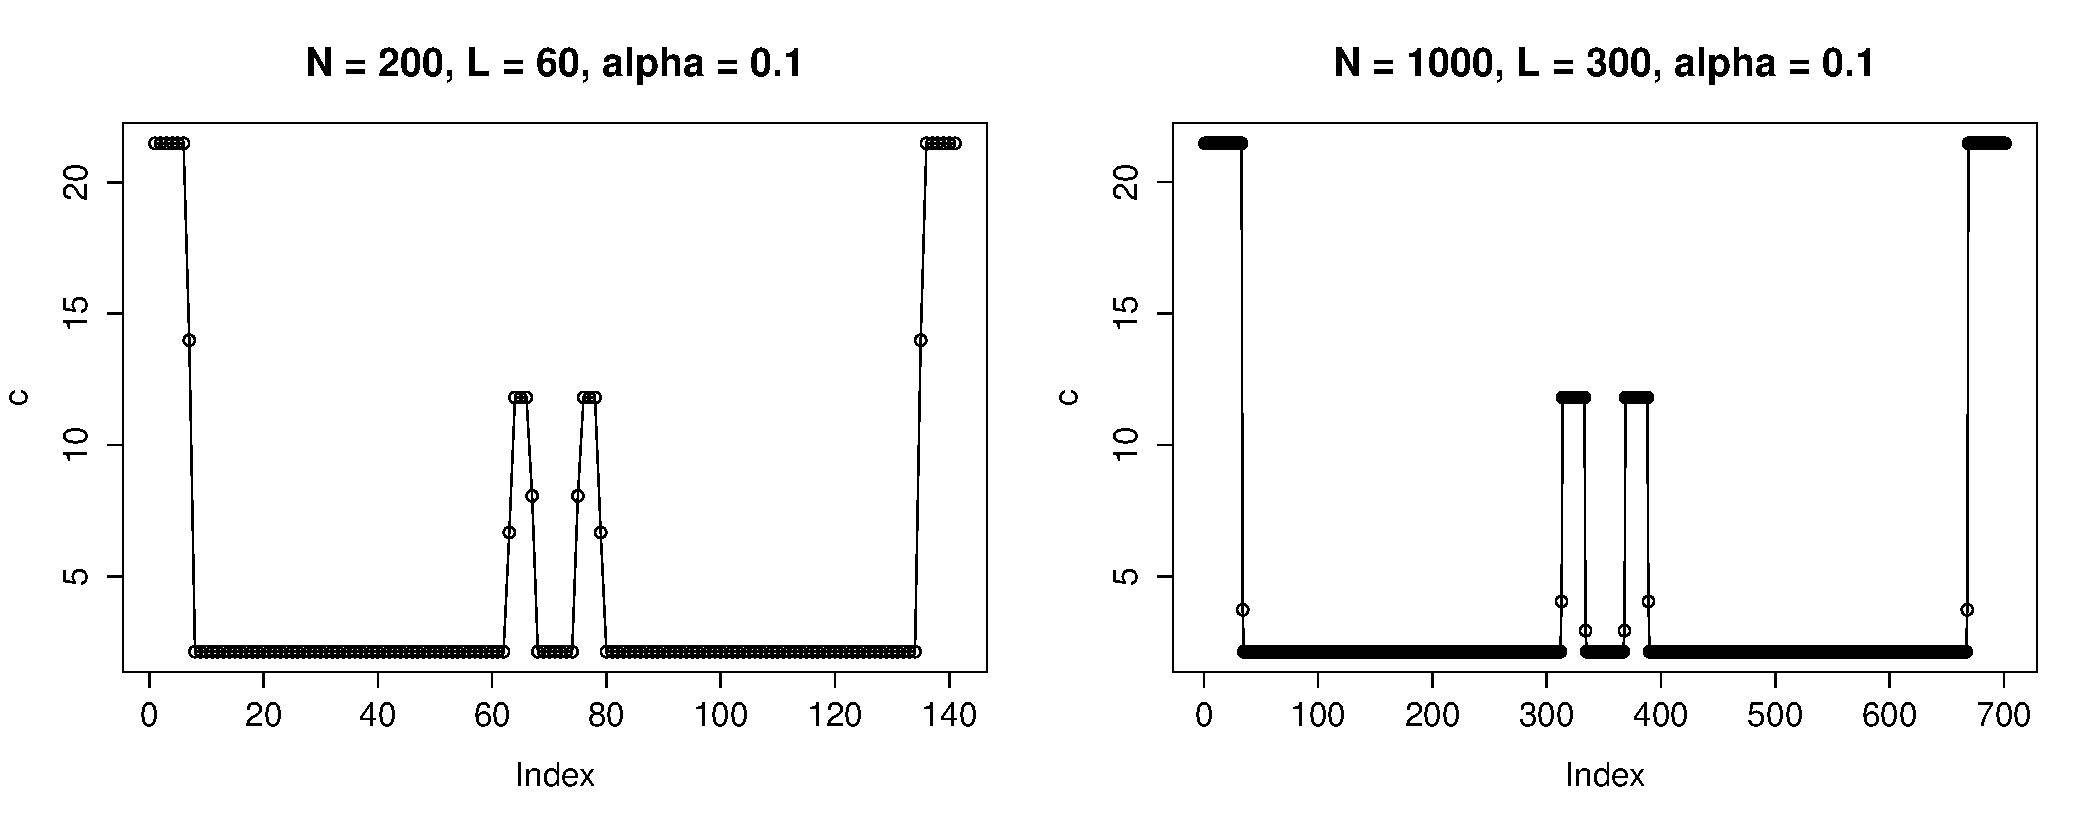
\includegraphics[width = \columnwidth]{scale.pdf}
		\caption{Два решения Задачи \ref{problem:quadtf} при одинаковом отношении $N$ к $L$}
		\label{img:scale}
	\end{figure}
	
	Схема эвристики следующая: зафиксируем параметр масштаба $0 < \gamma < 1$ (на практике хорошими значениями $\gamma$ являются $0.5$ -- $0.7$), найдём решение задачи при $N_\gamma \approx \gamma N$, $L_\gamma \approx \gamma L$, $\alpha_\gamma = \alpha$, после чего растянем решение задачи меньшего порядка для выбора начального рабочего множества и начальной точки. Таким образом, при использовании данной эвристики получаем рекурсивный алгоритм, который уменьшает размерность задачи в $\gamma$ раз до тех пор, пока $K$ не станет достаточно малым для использования первой стратегии.
	
\end{enumerate}

\section{Численный эксперимент} \label{sect:numeric}
Ниже приведём численное сравнение эффективности полученных с помощью алгоритма \ref{alg:solveqw} весов в задаче оценки сигнала рядом конечного ранга методом Oblique Cadzow \cite{Zvonarev2015}. Сравнение было проведено на примере синуса.

Был взят сигнал $\tsS = (s_{1}, \ldots, s_N)$ длины $N = 40$ и ранга $r=2$, имеющий вид:
\begin{equation*}
%\label{eq:signal}
s_{k} = 5\sin{\frac{2 \pi k}{6}}, \quad k = 1, \ldots, N,
\end{equation*}
и рассматривался ряд вида $\tsX = \tsS + \tsN$, где $\tsN$ --- гауссовский белый шум с нулевым средним и единичной дисперсией. Точность оценки сигнала $\widehat\tsS$ измерялась с помощью корня из среднего по точкам ряда и по 1000 реализациям ряда среднеквадратического отклонения (СКО) от сигнала $\tsS$. Эту меру будем называть RMSE (root mean-square error) оценки сигнала. В качестве меры скорости сходимости алгоритма Oblique Cadzow используется среднее число итераций до остановки. Длина окна зафиксирована равной $L = 20$. Был использован следующий критерий остановки метода Oblique Cadzow: $\frac{\|\calT_L^{-1}(\bfY_k) - \calT_L^{-1}(\bfY_{k + 1})\|^2}{N} < 10^{-8}$. Рассматривались веса, полученные Алгоритмом \ref{alg:solveqw} (тип I) и прежним методом замены нулей на $\alpha$ \cite[Proposition 5]{Zvonarev2015} (тип II). Результаты сравнения между весами одного типа при различных $\alpha$ являются значимыми при уровне значимости 5\%.

Результаты сравнения приведены в Таблице \ref{fintable}. Заметим, что результаты при $\alpha = 1$ и $\alpha = 2^{-5}, 2^{-6}, 2^{-7}, 2^{-8}$ совпадают, так как совпадают матричные веса, полученные двумя различными методами. Также заметим, что заявленные соотношения между $\alpha$ и точностью оценивания, $\alpha$ и скоростью сходимости метода Oblique Cadzow выполняются и для нового метода.

\begin{table}[!hhh]
	\caption{Сравнение методов по RMSE и среднему числу итераций при различных $\alpha$ и алгоритмах получения весов (I, II).}\label{fintable}
	\begin{center}
		\begin{tabular}{|c|c|c|c|c|}
			\hline $\alpha$ & RMSE, I & RMSE, II & Iterations, I & Iterations, II \\ 
			\hline 1 & 0.3811 & 0.3811 & 8.44 & 8.44 \\ 
			\hline $2^{-1}$ & 0.3615 & 0.3682 & 8.67 & 8.71 \\ 
			\hline $2^{-2}$ & 0.3475 & 0.3529 & 9.76 & 9.55 \\ 
			\hline $2^{-3}$ & 0.3371 & 0.3388 & 11.97 & 11.61 \\ 
			\hline $2^{-4}$ & 0.3300 & 0.3293 & 14.73 & 15.95 \\ 
			\hline $2^{-5}$ & 0.3247 & 0.3247 & 24.37 & 24.37 \\ 
			\hline $2^{-6}$ & 0.3231 & 0.3231 & 39.95 & 39.95 \\ 
			\hline $2^{-7}$ & 0.3227 & 0.3227 & 67.86 & 67.86 \\ 
			\hline $2^{-8}$ & 0.3226 & 0.3226 & 116.87 & 116.87 \\ 
			%\hline $2^{-9}$ & 0.3226 & 0.3226 & 201.09 & 201.09 \\ 
			\hline 
		\end{tabular} 

	\end{center}
\end{table}

\section*{Заключение}

В работе был представлен новый подход к поиску весов в задаче взвешенной аппроксимации рядом конечного ранга. Задача была сформулирована в нескольких эквивалентных формулировках, каждая из которых используется при построении алгоритма решения задачи. Подробно рассмотрен сам алгоритм и все участвующие в нём шаги. Указаны особенности задачи, позволяющие получить быструю практическую реализацию алгоритма её решения. Численный эксперимент подтверждает свойства весов, которые требовались от них при формулировке задачи аппроксимации.

%\subsection{Решение подзадачи КП и нахождение множителей Лагранжа}
%
%Заметим, что в задаче \eqref{eq:j_positw} каждое ограничение затрагивает максимум две переменные, т.е. каждый столбец матрицы $\bfA$ содержит либо один, либо два ненулевых коэффициента, при этом обычно $m = |\sfW_k|$ велико и близко к $K$, а по свойствам Алгоритма \ref{alg:asm} матрица $\bfA$ --- полного ранга. Эту информацию можно использовать для построения эффективного с точки зрения вычислительной сложности решения.
%
%Для решения поставленной вспомогательной задачи \eqref{eq:subtask} есть явная формула обобщённого метода наименьших квадратов:
%\begin{equation*}
%P_k^\star = \overline \bfA (\overline \bfA^\rmT \bfG \overline \bfA)^{-1} \overline \bfA^\rmT G_k,
%\end{equation*}
%где матрица $\overline \bfA \in \sfR^{K \times (K-m)}$ состоит из столбцов, составляющих базис ортогонального дополнения к базису столбцов матрицы $\bfA$. К тому же, в случае задачи \eqref{eq:j_positw} матрица $\bfG = \bfS$ имеет специальный вид \eqref{eq:bfS}, а $\overline \bfA$ строится разряжённой, следовательно, соответствующие члены данного выражения могут быть быстро вычислены, при этом система линейных уравнений имеет малый порядок $K-m$, что при большом значении $m$ позволяет быстро найти решение.
%
%Множители Лагранжа, составляющие вектор $U = (u_i : i \in \sfW_k)^\rmT \in \sfR^{m}$, находятся из переопределенной системы линейных уравнений $\bfA U =  \bfG P_k - G_K = R = (r_1, \ldots, r_K)^\rmT$, при этом вектор $R \in \text{span}(A_1, \ldots, A_m)$. Аналогично, решение можно найти быстро, используя информацию о том, что каждый столбец $\bfA$ содержит максимум два ненулевых компонента.
%
%Для этого построим неориентированный граф $\sfG=(\sfV, \sfE)$, где множество вершин $\sfV = \{1, 2, \ldots, K\}$, а множество рёбер $\sfE = \{e_i : i \in \sfW_k \}$ строится следующим образом: если $i$-й столбец матрицы $A_i = (a_{i, 1}, \ldots, a_{i, K})^\rmT$ содержит два ненулевых коэффициента $a_{i,k}$ и $a_{i,l}$, то $i$-е ребро соединяет вершины $k$ и $l$, то есть $e_i = (k, l)$; если же ребро содержит только один ненулевой коэффициент $a_{i,k}$, то $i$-е ребро представляет из себя петлю из вершины $k$ в вершину $k$, т.е. $e_i=(k, k)$. Назовём такой граф \emph{графом подзадачи} \eqref{eq:subtask}.
%
%Разбиение графа $\sfG$ на компоненты связности соответствует приведению матрицы $\bfA$ к блочно-диагональному виду. Такое разбиение множества вершин $\sfV$ = $\bigcup_{i=1}^{s} \sfV_i$ на $s$ подмножеств, где каждое множество вершин $\sfV_i$ вместе с соответствующим подмножеством рёбер $\sfE_i$ является связным графом $\sfG_i$, и при этом среди $\sfE$ не существует ребра, связывающего две разные компоненты, может быть построено, например, используя алгоритм поиска в глубину (DFS), см. \cite{cormen2009introduction}.
%
%Существует следующее простое утверждение о графе $\sfG_i$.
%\begin{proposition}
%Каждый граф $\sfG_i$ является либо деревом, либо графом с одним циклом.
%\end{proposition}
%\begin{proof}
%Пусть $l_i$ = $|\sfV_i|$. Так как $\sfG_i$ --- связный подграф, то он содержит минимум $l_i - 1$ вершину, то есть $|\sfE_i| \ge l_i - 1$. С другой стороны, каждому ребру из $\sfE_i$ соответствует столбец матрицы $\bfA$, у которого коэффициенты на всех индексах вне $\sfV_i$ гарантированно нулевые. Так как по предположению матрица $\bfA$ содержит линейно-независимые столбцы, получаем, что $\sfE_i \le l_i$.
%\end{proof}
%
%Рассмотрим каждую компоненту связности $\sfG_i$ по отдельности, и для них опишем алгоритм поиска матрицы $\overline \bfA$ и решения системы $\bfA U = R$.
%\subsection{Метод поиска множителей Лагранжа}
%Заметим простой факт: если некоторая вершина $k$ является листом, то есть существует только одно ребро $e_j = (l, k)$, ведущее в эту вершину, то коэффициент $u_j = r_k / a_{i, k}$, после чего $j$-е ребро можно удалить и перейти к решению системы $\widehat \bfA \widehat U = \widehat R$, где $\widehat \bfA = [A_i : i \in \sfW_k \setminus \{j \}]$, $\widehat U = (u_i : i \in \sfW_k \setminus \{j \})$, $\widehat R = R - u_j A_j$. Соответственно, быстрый алгоритм решения представляет из себя последовательное сокращение дерева путем ``отрезания'' листьев и нахождения решения системы.
%
%Схема алгоритма следующая: с помощью DFS проверим, содержит ли $\sfG_i$ цикл. Если нет (то есть $\sfG_i$ является деревом), то соответствующее последовательное сокращение дерева можно реализовать внутри обхода дерева с помощью DFS. В том случае, когда $\sfG_i$ содержит цикл, найдём его и пометим ребра, входящие в него. Затем из каждой вершины, лежащей в цикле, запустим описанный ранее спуск в глубину с сокращением (естественно, исключая вершины в цикле). В итоге, получим коэффициенты вектора $U$ для всех индексов, соответствующие ребра которых не лежат в цикле, а лежат в исходящих деревьях. Оставшаяся система линейных уравнений после перенумерации сводится к решению системы с циклической ленточной матрицей ширины $2$. За пояснениями см. \cite{cormen2009introduction}, \footnote{Какая-нибудь подходящая книга по разряженым матрицам}. %Данную систему можно решить за линейное время с помощью метода Гаусса, но, в целом, обход графа в глубину и решение таких систем лежат вне области данной статьи. 
%\subsection{Метод поиска матрицы-дополнения}
%Покажем, как можно найти матрицу $\overline \bfA$, базис из столбцов которой является ортогональным дополнением к базису $\bfA$. Это можно сделать, предъявив ортогональную матрицу порядка $K \times (K-m)$, каждый столбец которой ортогонален всем столбцам матрицы $\bfA$.
%
%Рассмотрим компоненту связности $\sfG_i$. Если она является графом с одним циклом, то дополнение к соответствующему базису столбцов является пустым. Если же $\sfG_i$ является деревом, то линейная оболочка столбцов матрицы $\bfA$, соответствующих ребрам, лежащим в $\sfE_i$, имеет размерность $l_{i-1}$, где $l_i = | \sfV_i |$, а дополнение до линейного подпространства $\sfR^{\sfV_i}$ имеет размерность $1$, где $\sfR^{\sfV_i}$ --- подпространство $\sfR^K$ с элементами, у которых элементы на лежащих в $\sfV_i$ индексах произвольные, и нулевые для всех остальных индексов.
%
%Тогда если мы рассмотрим вектор $\overline A_i = (\overline a_{i, 1}, \ldots, \overline a_{i, K})^\rmT$, лежащий в дополнении до $\sfR^{\sfV_i}$, то для любого ребра $e_j= (l,k)$, лежащего в $\sfE_i$, должно выполняться условие ортогональности: $\overline a_{i, l} a_{j, l} + \overline a_{i, k} a_{j, k} = 0$.
%
%Алгоритм поиска следующий: для всех $j \notin \sfV_i$ положим $\overline a_{i, j} = 0$. Выберем произвольный индекс $k \in \sfV_i$, положим $\overline a_{i, k} = 1$, после чего запустим алгоритм спуска по дереву в глубину из вершины $k$ по компоненте связности $\sfG_i$. При рассмотрении ребра $e_j$, идущего из посещённой алгоритмом вершины $k$ в непосещённую $l$, положим
%\begin{equation*}
%\overline a_{i, l} = -\frac{\overline a_{i, k} a_{j, k}}{a_{j, l}}.
%\end{equation*}
%
%Таким образом, получим матрицу $\overline \bfA = [\overline A_i \; | \sfG_i \; \text{является деревом}]$, удовлетворяющую всем нужным свойствам.
%
%\subsection{Эвристика выбора начального приближения при небольшой размерности задачи}
%Оставшийся шаг --- описать пункт 1 в Алгоритме \ref{alg:asm}, применяемом при решении задачи \eqref{eq:j_positw}. На самом деле, на первом шаге можно достаточно точно подобрать рабочее множество $\sfW_0$, которое во многом совпадает с итоговым, соответствующим точке минимума, при этом важно, чтобы начальная точка удовлетворяла всем ограничениям.
%
%Рассмотрим две таких эвристики: первая хорошо работает в том случае, когда $K$ мало, вторая позволяет использовать решение задачи меньшего порядка для нахождения начального рабочего множества. Вначале рассмотрим первую эвристику.
%
%Посмотрим на набор ограничений в задаче \eqref{eq:j_positw}. Ограничения \eqref{eq:positw_symm} задают симметричность весов --- они обязательно входят в любое рабочее множество. Ограничение \eqref{eq:positw_notnull}, если оно входит в рабочее множество, устанавливает равенство нулю в точке с индексом $j$. Ограничения \eqref{eq:positw_min} устанавливают вес точки, равный минимально допустимому при заданном параметре $\alpha$, а \eqref{eq:positw_max} --- максимально возможный и равный $c_j$.
%
%Эвристика заключается в том, чтобы для точек $1$, $2, \ldots, j-1$, $j + 1, \ldots, \ldots, \lceil K/2\rceil$ назначить первым $0 \le t \le \lceil K/2\rceil - 1$ максимальный вес, а оставшимся --- минимальный, после чего решить соответствующую задачу КП.  Графически, используя терминологию текущего раздела, такие ограничения можно изобразить следующим образом (на графе изображён случай $j = 1$, положение вершин соответствует реальному решению задачи, сплошные рёбра соответствуют ограничениям вида \eqref{eq:positw_symm}, рёбра точечным пунктиром --- \eqref{eq:positw_max}, прерывистым пунктиром --- \eqref{eq:positw_min}, рёбра на рисунке ориентированы согласно порядку обхода графа из первой вершины):
%
%\begin{center}
%\begin{tikzpicture}[scale=0.85]
%\node[shape=circle,draw=black] (A) at (0,3) {1};
%\node[shape=circle,draw=black] (B) at (1.4,3) {2};
%\node[shape=circle,draw=black] (C) at (2.8, 3) {\ldots};
%\node[shape=circle,draw=black] (D) at (4.5,3) {$t + 1$};
%\node[shape=circle,draw=black] (E) at (5.7, 0) {$t + 2$};
%\node[shape=circle,draw=black] (F) at (7.4,0) {\ldots} ;
%\node[shape=circle,draw=black] (G) at (9.4,0) {$K - t + 1$} ;
%\node[shape=circle,draw=black] (H) at (10.3,3) {$K - t$} ;
%\node[shape=circle,draw=black] (I) at (11.8,3) {\ldots} ;
%\node[shape=circle,draw=black] (J) at (13.3,3) {$K - 1$} ;
%\node[shape=circle,draw=black] (K) at (14.8,3) {$K$} ;
%
%\path [->, dotted](A) edge node[left] {} (B);
%\path [->, dotted](A) edge[bend left = 30] node[left] {} (C);
%\path [->, dotted](A) edge[bend left = 30] node[left] {} (D);
%\path [->, dashed](A) edge node[left] {} (E);
%\path [->, dashed](A) edge[bend left = 5] node[left]{} (F);
%\path [->](E) edge[bend right = 30] node[left]{} (G);
%\path [->](D) edge node[left] {} (H);
%\path [->](C) edge[bend right = 35] node[left]{} (I);
%\path [->](B) edge[bend right = 30] node[left]{} (J);
%\path [->](A) edge[bend right = 70] node[left]{} (K);
%
%\end{tikzpicture}
%\end{center}
%
%
%%$t$ будем перебирать в цикле жадно, начиная с $0$, пока значение целевой функции не начнет снова возрастать или не достигнет $0 \le t \le \lceil K/2\rceil - 1$.
%Так как угадать значение $t$ трудно, опишем жадный алгоритм перебора $t$:
%\begin{algorithm}
%	\label{alg:beginheuristic}
%	\textbf{Вход}: текущий индекс максимального веса $j$.
%	
%	\textbf{Результат}:
%	Начальное рабочее множество ограничений $\sfW_0$ и стартовая точка $X_0$.
%	
%	\begin{enumerate}
%	    \item Положить $f_0 = +\infty$.
%	    \item Вычислить вектор индексов $Z = (1, 2, \ldots, j-1, j+1, \ldots, \lceil K/2\rceil)$.
%		\item Для $t = 1, 2, \ldots, \lceil K/2\rceil - 1$:
%		\begin{enumerate}
%		\item Решить следующую задачу квадратичного программирования, вычислить значение целевой функции $f_t(C^\star_t)$ и точки минимума $C^\star_t$, запомнить рабочее множество $\widehat \sfW_t$:
%		\begin{gather*}
%f_t(C) = \frac{1}{2} C^\rmT \bfS C - L_K^T C \to \min_{C} \quad \text{при условиях} \\
%c_i = c_{K - i + 1}, \; i = 1,\ldots, \lceil K/2\rceil, \\ 
%c_{z_i} - \alpha c_j = 0, \; i = t+1, \ldots, \lceil K/2\rceil - 1\\
%c_{z_i} -  c_i = 0, \; i = 1,\ldots, t.
%\end{gather*}
%        \item Если $f_t > f_{t-1}$, то вернуть набор ограничений с предыдущей итерации $\sfW_0 = \widehat \sfW_{t-1}$ и точку $X_0 = C_0 = C^\star_{t-1}$.
%		\end{enumerate}
%	\item Вернуть набор ограничений с последней итерации $\widehat \sfW_{\lceil K/2\rceil - 1}$ и точку $X_0 = C_0 = C_{\lceil K/2\rceil - 1}$. \footnote{Этот шаг выполняется только в том случае, когда жадный алгоритм не встретил ``излом'' целевой функции}
%\end{enumerate}
%\end{algorithm}
%Заметим, что при использовании теории данного раздела для нахождения начальной точки по формуле взвешенного метода наименьших квадратов требуется решать систему линейных уравнений порядка $1$.
%
%\subsection{Эвристика выбора начального приближения при большой размерности задачи}
%Второй алгоритм выбора начальной точки основан на том, что решения задач при (примерно) одинаковом отношении $N$ к $L$ и одинаковом $\alpha$ схожи. Например, на Рисунке \ref{img:scale} изображены два отнормированных (умноженных на $N$) решения Задачи \ref{problem:quadtf} при $N = 200$, $L = 60$, $\alpha = 0.1$ и $N = 1000$, $L = 300$, $\alpha = 0.1$ соответственно.
%
%\begin{figure}[!hhh]
%	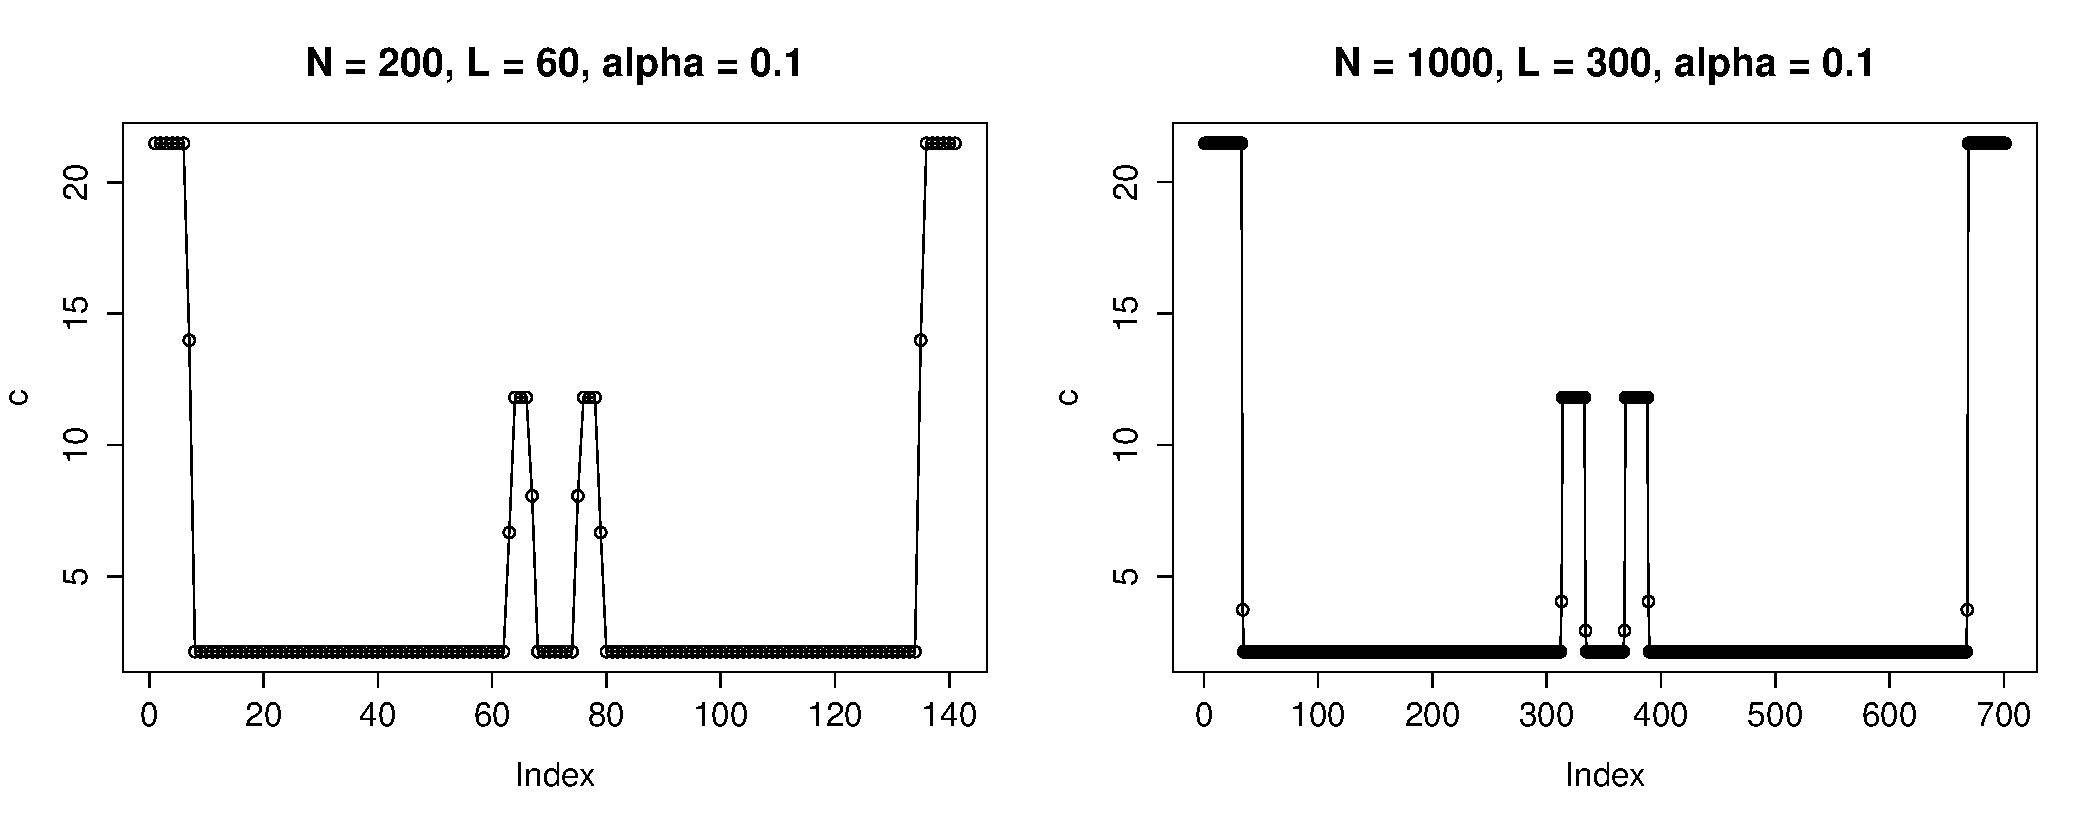
\includegraphics[width = \columnwidth]{scale.pdf}
%	\caption{Два решения Задачи \ref{problem:quadtf} при одинаковом отношении $N$ к $L$}
%	\label{img:scale}
%\end{figure}
%
%Схема эвристики следующая: зафиксируем параметр масштаба $0 < \gamma < 1$ (на практике хорошими значениями $\gamma$ являются $0.5$ -- $0.7$), найдём решение задачи при $N_\gamma \approx \gamma N$, $L_\gamma = \approx \gamma L$, $\alpha_\gamma = \alpha$, после чего используем решение задачи меньшего порядка для выбора начального рабочего множества и начальной точки. Формально, алгоритм выглядит так:
%
%\begin{algorithm}
%	\label{alg:bigheuristic}
%	\textbf{Вход}: текущий индекс максимального веса $j$, параметр $\gamma$.
%	
%	\textbf{Результат}:
%	Начальное рабочее множество ограничений $\sfW_0$ и стартовая точка $X_0$.
%	
%	\begin{enumerate}
%		\item Положить $K\gamma = [\gamma K ]$, $L\gamma = [\gamma L ]$, $N_\gamma = L_\gamma + K_\gamma - 1$.
%		\item Определить функцию перехода к ``уменьшенным'' координатам $s(i) = [\frac{(i - 1)(K_\gamma - 1)}{K - 1}~+~1]$.
%		\item Положить $j_\gamma = s(j)$.
%		\item Найти масштабированное решение $C_\gamma = (c_{\gamma, 1}, \ldots, c_{\gamma, K_\gamma})^\rmT$ задачи \eqref{eq:j_positw} при $K = K_\gamma$, $L = L_\gamma$, $\alpha = \alpha$, $j = j_\gamma$.
%		\item Положить в рабочее множество $\sfW$ индексы всех ограничений вида \eqref{eq:positw_symm}.
%		%\item Вычислить вектор индексов $Z = (1, 2, \ldots, j-1, j+1, \ldots, \lceil K/2\rceil)$.
%		\item Для $i = 1, 2, \ldots, \lceil K/2\rceil$:
%		\begin{enumerate}
%			\item Если $i = j$, то пропустить итерацию, иначе вычислить $i_\gamma = s(i)$.
%			\item Если $c_{\gamma, i_\gamma} = c_{\gamma, j_\gamma}$, то положить $\sfW \leftarrow \sfW \cup \text{index}(\{c_j - c_i \ge 0\})$, и перейти к следующей итерации.
%			\item Если $c_{\gamma, i_\gamma} - \alpha c_{\gamma, j_\gamma} = 0$, то положить $\sfW \leftarrow \sfW \cup \text{index}(\{c_i - \alpha c_j \ge 0\})$.
%		\end{enumerate}
%		
%		\item Для $k = 1, 2, \ldots$:
%		\begin{enumerate}
%			\item Решить следующую задачу квадратичного программирования, вычислить значение точки минимума $C^\star$:
%			\begin{gather*}
%			\frac{1}{2} C^\rmT \bfS C - L_K^T C \to \min_{C} \quad \text{при условиях} \\
%			A_i^\rmT C = 0, \quad i \in \sfW, 
%			\end{gather*}
%			\item Проверить на точке $C^\star$ все условия вида \eqref{eq:positw_min} и \eqref{eq:positw_max}. Если все они выполняются, то ответ --- $X_0 = C^\star$ и $\sfW_0 = \sfW$, иначе добавить к рабочему множеству $W$ индекс ограничения, которое не выполняется.
%		\end{enumerate}
%	\end{enumerate}
%\end{algorithm}
%
%Заметим, что п. 7 Алгоритма \ref{alg:beginheuristic}, необходимый для того, чтобы получить корректную начальную точку, совершит не более $\lceil K/2 \rceil$ итераций вследствие того, что каждая итерация уменьшает размерность линейной оболочки, в которой лежит начальная точка $C^\star$, на единицу.
%
%Таким образом, при использовании данной эвристики получаем рекурсивный алгоритм, который уменьшает размерность задачи в $\gamma$ раз до тех пор, пока $K$ не станет достаточно малым для использования первой эвристики.
%\begin{theorem} \label{th:eqivqw}
%	Задачи \eqref{eq:nonnegatqw} и \eqref{eq:positw} эквивалентны.
%\end{theorem}
%\begin{proof}
%	Для доказательства эквивалентности нужно показать, что по индексу $j$ можно построить вектор $\widehat C$ такой, что $f_j \ge f(\widehat C)$, и наоборот: по вектору $\widehat C$ найти такой индекс $j$, что $f(\widehat C) \ge f_j$.
%	
%	Рассмотрим оба пункта доказательства.
%	\begin{enumerate}
%		\item Пусть $j$ --- индекс максимального веса, $\widetilde C_j = \widetilde C_j^*$ --- решение соответствующей задачи \eqref{eq:j_positqw}. Тогда рассмотрим следующий вектор $\widehat C$: $\hat c_i = \tilde c_i$, $i = 1, \ldots, j-1, j+1, \ldots, K$, $c_\text{max} = \tilde c_\text{max}$, $\hat c_j = 0$. Так как по построению $\bfH_j \widetilde C_j = \bfH \widehat C$, то целевые функции равны. Выполнение свойств \eqref{eq:nonnegatqw_cond} очевидным образом следует из условий \eqref{eq:j_positqw_cond}.
%		\item Вначале рассмотрим вектор $\widehat C$, и найдём такой индекс $j$ и вектор $\widetilde C_j$, что $f(\widehat C) = f_j(\widetilde C_j)$. В качестве $j$ возьмём $j = \argmax_i c_\text{max} - \hat c_i$. Тогда $\tilde c_\text{max} = c_\text{max} - \hat c_j$, а $\tilde c_i = \tilde c_\text{max} - c_\text{max} + \hat c_i = \hat c_i - \hat c_j$, $i = 1, \ldots, j-1, j+1, \ldots, K$. Заметим, что $\tilde c_\text{max} \le c_\text{max}$. Из того, что $c_i = c_\text{max} - \hat c_i = c_\text{max} - \hat c_j + \hat c_j - \hat c_i = \tilde c_\text{max} + \hat c_j - \hat c_i =$ $\tilde c_\text{max} - \tilde c_i$, что эквивалентно $\bfH_j \widetilde C_j = \bfH \widehat C$, следует равенство целевых функций задачи \eqref{eq:nonnegatqw} и вспомогательной задачи \eqref{eq:j_positqw}.
%		
%		Покажем, что $\tilde c_\text{max} \ge 0$. $\tilde c_\text{max} = c_\text{max} - \hat c_j \ge \hat c_j (1/(1 - \alpha) - 1) \ge 0$, если $\alpha < 1$. Если же $\alpha = 1$, то все $\hat c_i = 0$, и $\tilde c_\text{max} = c_\text{max} \ge 0$. $\tilde c_i \ge 0$, $i = 1, \ldots, K$, $i \neq j$ следует из того, что $\hat c_j$ --- минимальное среди всех $\hat c_i$, $i = 1, \ldots, K$. Последние неравенства проверяются следующим способом: $(1 - \alpha) \tilde c_\text{max} - \tilde c_i = (1 - \alpha)(c_\text{max} - \hat c_j) - \hat c_i + \hat c_j = $ $(1 - \alpha)c_\text{max} - \hat c_i + \alpha \hat c_j \ge 0$.
%		
%		Заметим, что $f_j = f_j(\widetilde C_j^*) \le f_j(\widetilde C_j)$, что и требовалось доказать.
%	\end{enumerate}
%\end{proof}

%\section{Случай нормы $\|X\|_\infty$}
%Покажем, что данная задача сводится к задаче линейного программирования с линейными ограничениями с помощью добавления вспомогательных переменных.
%
%Рассмотрим $\omega \in \sfR$ --- ещё один дополнительный параметр, который хранит значение целевой функции. Заметим, что при любых дополнительных условиях, любой матрице $\bfA \in \sfR^{N \times K}$, любого $\widetilde Y \in \sfR_N$, $\widetilde Y = (\tilde y_1, \ldots, \tilde y_N)^\rmT$, следующие задачи эквивалентны: 
%\begin{equation*}
%\|\bfA X - \widetilde Y \|_\infty \to \min_{X \in \sfR_K}
%\end{equation*}
%и 
%\begin{gather*}
%\omega \to \min_{X, \omega} \quad \text{при условиях} \\ \bfA X = Y = (y_1, \ldots, y_N)^\rmT, \quad y_i - \tilde y_i \le \omega, \quad y_i - \tilde y_i \ge -\omega, \quad i = 1, \ldots, N. 
%\end{gather*}
%
%Таким образом, в терминах линейного программирования задача \eqref{eq:commonw} в случае нормы $\|X\|_\infty$ переписывается следующим образом:
%\begin{gather*}
%\omega \to \min_{c_\text{max}, \, \hat c_1, \ldots, \hat c_K, \, \omega} \quad \text{при условиях} \\ \bfT \bfH \widehat C = Q = (q_1, \ldots, q_N)^\rmT, \quad q_i - 1 \le \omega, \quad q_i - 1 \ge -\omega, \quad i = 1, \ldots, N, \\
%c_\text{max} \ge 0, \quad \hat c_j \ge 0, \quad (1 - \alpha) c_\text{max} - \hat c_j \ge 0, \quad j = 1, \ldots, K.
%\end{gather*}
%
%\section{Случай нормы $\|X\|_1$}
%Аналогично предыдущему случаю, задача \eqref{eq:commonw} может быть записана в терминах линейного программирования.
%
%Для этого заметим следующее: если ввести $2N$ дополнительных переменных \\ $\kappa_1, \ldots, \kappa_N$, $\theta_1, \ldots, \theta_N \in \sfR$, то при любых дополнительных условиях, любой матрице $\bfA \in \sfR^{N \times K}$, любого $\widetilde Y \in \sfR_N$, $\widetilde Y = (\tilde y_1, \ldots, \tilde y_N)^\rmT$, следующие задачи эквивалентны: 
%\begin{equation*}
%\|\bfA X - \widetilde Y \|_1 \to \min_{X \in \sfR^K}
%\end{equation*}
%и 
%\begin{gather*}
%\sum_{i = 1}^N (\kappa_i + \theta_i) \to \min_{X, \, \kappa_1, \ldots, \kappa_N, \, \theta_1, \ldots, \theta_N} \quad \text{при условиях} \\ \bfA X = Y = (y_1, \ldots, y_N)^\rmT, \quad y_i - \tilde y_i = \kappa_i - \theta_i, \quad \kappa_i \ge 0, \quad \theta_i \ge 0, \quad i = 1, \ldots, N. 
%\end{gather*}
%
%В итоге, задача \eqref{eq:commonw} в терминах линейного программирования в случае нормы $\|X\|_1$ переписывается следующим образом:
%\begin{gather*}
%\sum_{i = 1}^N (\kappa_i + \theta_i) \to \min_{c_\text{max}, \, \hat c_1, \ldots, \hat c_K, \, \kappa_1, \ldots, \kappa_N, \, \theta_1, \ldots, \theta_N} \quad \text{при условиях} \\ \bfT \bfH \widehat C = Q = (q_1, \ldots, q_N)^\rmT,  \quad q_i - 1 = \kappa_i - \theta_i, \quad \kappa_i \ge 0, \quad \theta_i \ge 0, \quad i = 1, \ldots, N, \\
%c_\text{max} \ge 0, \quad \hat c_j \ge 0, \quad (1 - \alpha) c_\text{max} - \hat c_j \ge 0, \quad j = 1, \ldots, K.
%\end{gather*}

\bibliographystyle{gost705}
\inputencoding{cp1251}
\bibliography{weights}
\end{document}
